% Gallery figure source
% Summary: Linkage as a breakpoint problem. Two sites are separated by recombination only when a crossover breakpoint falls between them. Nearby sites have a short interval between them and tend to remain in the same ancestry block, while distant sites have a larger interval between them and are more likely to have different local trees.
\documentclass[tikz,border=6pt]{standalone}
% Shared color palette
\usepackage[T1]{fontenc}
\usepackage[utf8]{inputenc}
\usepackage{lmodern}
\usepackage{microtype}
\usepackage{amsmath,amssymb,mathtools}
\usepackage{xcolor}
\usepackage{tikz}
\usetikzlibrary{arrows.meta,positioning,calc,fit,backgrounds,decorations.pathreplacing,shapes.geometric,shadows.blur}

\definecolor{mainblue}{RGB}{42,85,132}
\definecolor{deepgreen}{RGB}{30,105,70}
\definecolor{burntorange}{RGB}{190,90,25}
\definecolor{softgray}{RGB}{245,246,248}
\definecolor{darkgray}{RGB}{70,70,70}
\definecolor{violet}{RGB}{110,70,150}

\newcommand{\given}{\,|\,}
\newcommand{\Ne}{N_{e}}
\newcommand{\ARG}{\mathrm{ARG}}
\newcommand{\MRCA}{\mathrm{MRCA}}
\newcommand{\GMRCA}{\mathrm{GMRCA}}

% Shared TikZ styles
\tikzset{
  tip/.style={circle,fill=black,inner sep=1.6pt},
  nodept/.style={circle,fill=black,inner sep=1.4pt},
  sampled/.style={rectangle,fill=black,inner sep=2.2pt},
  branch/.style={line width=0.8pt},
  retic/.style={circle,draw=burntorange,fill=burntorange!25,line width=0.8pt,inner sep=2.0pt},
  event/.style={circle,draw=mainblue,fill=mainblue!15,line width=0.8pt,inner sep=1.8pt},
  arr/.style={-{Latex[length=2.0mm]},line width=0.8pt},
  faint/.style={line width=0.7pt,draw=gray!55},
  parentedge/.style={-{Latex[length=2.0mm]},line width=0.9pt,draw=burntorange},
  treeedge/.style={-{Latex[length=2.0mm]},line width=0.9pt,draw=black},
  segment/.style={line width=4pt,line cap=round},
  dashedretic/.style={-{Latex[length=2.0mm]},line width=0.9pt,draw=burntorange,dashed}
}


\begin{document}
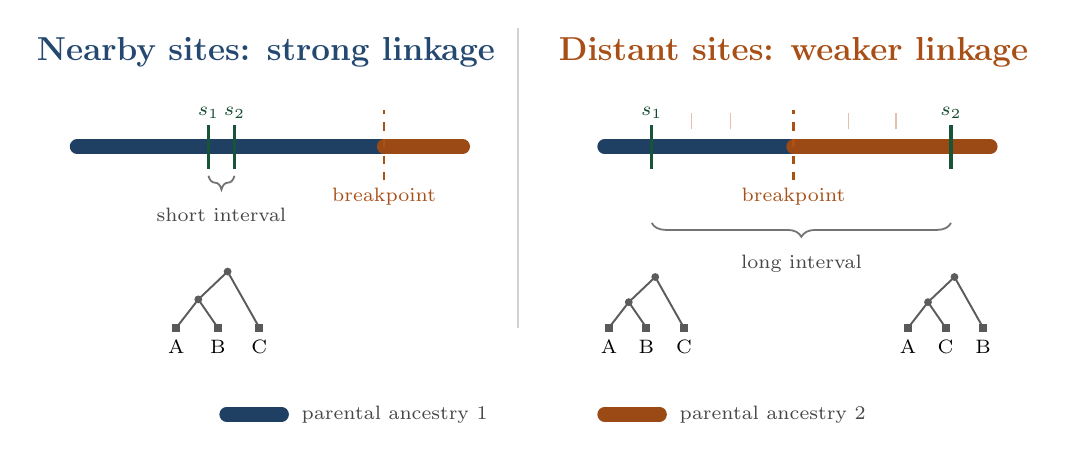
\begin{tikzpicture}[
  scale=1.0,
  paneltitle/.style={font=\bfseries\large},
  chrom/.style={line width=5.2pt,line cap=round},
  cut/.style={line width=.85pt,dashed,draw=burntorange!90!black},
  site/.style={line width=1.1pt,draw=deepgreen!80!black},
  intervalbrace/.style={decorate,decoration={brace,amplitude=5pt,mirror},line width=.65pt,draw=darkgray!75},
  note/.style={font=\small,align=center,text width=5.4cm,text=darkgray},
  smallnote/.style={font=\scriptsize,align=center,text=darkgray},
  treeicon/.style={line width=.7pt,draw=darkgray!88,line cap=round},
  tinode/.style={circle,fill=darkgray!88,inner sep=1.0pt},
  ttip/.style={rectangle,fill=darkgray!90,inner sep=1.45pt}
]

\draw[chrom,draw=mainblue!75!black] (2.35,-1.05)--(3.05,-1.05);
\node[font=\scriptsize,anchor=west,text=darkgray] at (3.18,-1.05) {parental ancestry 1};

\draw[chrom,draw=burntorange!82!black] (7.15,-1.05)--(7.85,-1.05);
\node[font=\scriptsize,anchor=west,text=darkgray] at (7.98,-1.05) {parental ancestry 2};

\begin{scope}
  \node[paneltitle,text=mainblue!85!black] at (2.85,3.55)
    {Nearby sites: strong linkage};

  \draw[chrom,draw=mainblue!75!black] (0.45,2.35)--(4.35,2.35);
  \draw[chrom,draw=burntorange!82!black] (4.35,2.35)--(5.35,2.35);

  \draw[cut] (4.35,1.92)--(4.35,2.82);
  \node[smallnote,text=burntorange!88!black] at (4.35,1.72)
    {breakpoint};

  \coordinate (LsiteOne) at (2.12,2.35);
  \coordinate (LsiteTwo) at (2.45,2.35);

  \draw[site] ($(LsiteOne)+(0,-0.28)$)--($(LsiteOne)+(0,0.28)$);
  \draw[site] ($(LsiteTwo)+(0,-0.28)$)--($(LsiteTwo)+(0,0.28)$);

  \node[font=\scriptsize,text=deepgreen!70!black] at (2.12,2.78) {$s_1$};
  \node[font=\scriptsize,text=deepgreen!70!black] at (2.45,2.78) {$s_2$};

  \draw[intervalbrace] (2.12,1.98)--(2.45,1.98)
    node[midway,below=8pt,font=\scriptsize,text=darkgray] {short interval};

  \begin{scope}[xshift=1.65cm,yshift=0.05cm,scale=.62]
    \coordinate (Lr) at (1.15,1.15);
    \coordinate (Ln) at (0.55,0.58);
    \coordinate (La) at (0.10,0.00);
    \coordinate (Lb) at (0.95,0.00);
    \coordinate (Lc) at (1.80,0.00);

    \draw[treeicon] (Lr)--(Ln)--(La);
    \draw[treeicon] (Ln)--(Lb);
    \draw[treeicon] (Lr)--(Lc);

    \foreach \p in {Lr,Ln}{
      \node[tinode] at (\p) {};
    }

    \foreach \p/\lab in {La/A,Lb/B,Lc/C}{
      \node[ttip] at (\p) {};
      \node[below=1pt,font=\scriptsize] at (\p) {\lab};
    }
  \end{scope}
\end{scope}

\draw[gray!35,line width=.6pt] (6.05,0.05)--(6.05,3.85);

\begin{scope}[xshift=6.70cm]
  \node[paneltitle,text=burntorange!88!black] at (2.85,3.55)
    {Distant sites: weaker linkage};

  \draw[chrom,draw=mainblue!75!black] (0.45,2.35)--(2.85,2.35);
  \draw[chrom,draw=burntorange!82!black] (2.85,2.35)--(5.35,2.35);

  \draw[cut] (2.85,1.92)--(2.85,2.82);
  \node[smallnote,text=burntorange!88!black] at (2.85,1.72)
    {breakpoint};

  \coordinate (RsiteOne) at (1.05,2.35);
  \coordinate (RsiteTwo) at (4.85,2.35);

  \draw[site] ($(RsiteOne)+(0,-0.28)$)--($(RsiteOne)+(0,0.28)$);
  \draw[site] ($(RsiteTwo)+(0,-0.28)$)--($(RsiteTwo)+(0,0.28)$);

  \node[font=\scriptsize,text=deepgreen!70!black] at (1.05,2.78) {$s_1$};
  \node[font=\scriptsize,text=deepgreen!70!black] at (4.85,2.78) {$s_2$};

  \draw[intervalbrace] (1.05,1.38)--(4.85,1.38)
    node[midway,below=8pt,font=\scriptsize,text=darkgray] {long interval};

  \foreach \x in {1.55,2.05,3.55,4.15}{
    \draw[line width=.45pt,draw=burntorange!38] (\x,2.57)--(\x,2.78);
  }

  \begin{scope}[xshift=0.45cm,yshift=0.05cm,scale=.56]
    \coordinate (Rar) at (1.15,1.15);
    \coordinate (Ran) at (0.55,0.58);
    \coordinate (Raa) at (0.10,0.00);
    \coordinate (Rab) at (0.95,0.00);
    \coordinate (Rac) at (1.80,0.00);

    \draw[treeicon] (Rar)--(Ran)--(Raa);
    \draw[treeicon] (Ran)--(Rab);
    \draw[treeicon] (Rar)--(Rac);

    \foreach \p in {Rar,Ran}{
      \node[tinode] at (\p) {};
    }

    \foreach \p/\lab in {Raa/A,Rab/B,Rac/C}{
      \node[ttip] at (\p) {};
      \node[below=1pt,font=\scriptsize] at (\p) {\lab};
    }
  \end{scope}

  \begin{scope}[xshift=4.25cm,yshift=0.05cm,scale=.56]
    \coordinate (Rbr) at (1.15,1.15);
    \coordinate (Rbn) at (0.55,0.58);
    \coordinate (Rba) at (0.10,0.00);
    \coordinate (Rbc) at (0.95,0.00);
    \coordinate (Rbb) at (1.80,0.00);

    \draw[treeicon] (Rbr)--(Rbn)--(Rba);
    \draw[treeicon] (Rbn)--(Rbc);
    \draw[treeicon] (Rbr)--(Rbb);

    \foreach \p in {Rbr,Rbn}{
      \node[tinode] at (\p) {};
    }

    \foreach \p/\lab in {Rba/A,Rbc/C,Rbb/B}{
      \node[ttip] at (\p) {};
      \node[below=1pt,font=\scriptsize] at (\p) {\lab};
    }
  \end{scope}
\end{scope}

\end{tikzpicture}
\end{document}
